\documentclass[8pt]{article}
\usepackage{graphicx}
	\setkeys{Gin}{width=0.4\textwidth}
\usepackage[a4paper]{geometry}
\usepackage{listings}
\twocolumn
\begin{document}
	\author{Jonathan Cancio \\ Oliver Atienza \\ Justin Balderas \\ 
	Reyster Fresco \\ Yna Ojeda \\ Ethan Tan \\ Marc Teves \\ Troy Valdez}
	\title{CS 131 MP2}
	\maketitle
	\section{Abstract}
	% Make sure to always have one sentence per line.
	Lorem ipsum dolor sit amet, consectetur adipiscing elit. Suspendisse et augue iaculis, bibendum nulla ut, cursus ante. Vivamus auctor posuere nisi, eget facilisis arcu consequat non. Vivamus semper arcu leo, ut rutrum nibh scelerisque a. Sed porta arcu id tortor maximus elementum. Duis at ante elit. Suspendisse sapien est, sollicitudin ac magna id, tristique tincidunt lorem. Nullam vulputate pretium elit, nec rutrum risus maximus ut. Donec purus nulla, vestibulum eu diam ac, feugiat dapibus erat. 
	\section{Introduction}
	Hello\cite{heath}
	\section{Methodology}

	\begin{figure}[h]
		\centering
		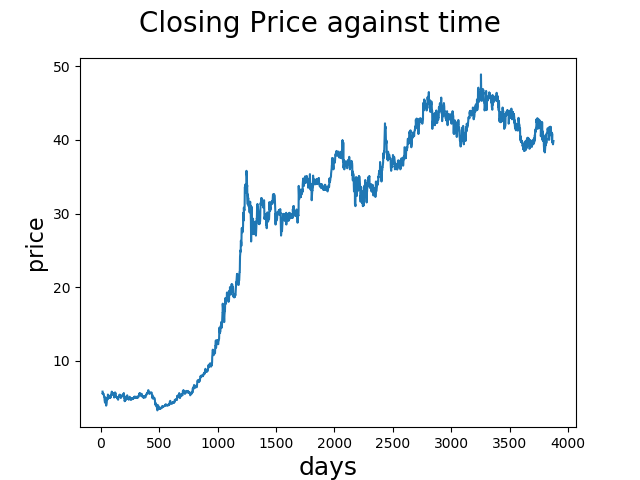
\includegraphics{ap_closing_price.png}
		\caption{Closing prices}
		\label{fig:close_price_graph}
	\end{figure}

	Take a look at Figure~\ref{fig:close_price_graph}. On the x-axis is
	\texttt{days} and the y-axis is \textbf{price}
	\subsection{Preprocessing}
	In this section we take a look at the data processing required to make the
	data workable.
		\subsubsection{Removing irrelevant companies}
		Go through each entry one by one and delete it if it's not one of the tracked companies.

	\section{Results}
	\section{Discussion}
	\section{Conclusion}
	\begin{thebibliography}{9}
		\bibitem{heath}
			Heath M.,

			\textit{Scientific Computing - An Introductory Survey}
	\end{thebibliography}
\end{document}
